\begin{frame}{(Continuous) Integration of scientific software}
    \framesubtitle{Hands on: overview}
    \begin{columns}
    \begin{column}{0.48\textwidth}
        \begin{block}{1. Repository preparation}
            A minimal repository representing an exemplary
            "status quo".
        \end{block}
        \begin{block}{2. Create a Docker image}
            Configure a reproducible testing environment.
        \end{block}
    \end{column}

    \begin{column}{0.48\textwidth}
        \begin{exampleblock}{3. Define CI pipeline through a YAML file}
            Define tests, how and when they are executed and what
            results to store.
        \end{exampleblock}
        \begin{block}{4. Setup your own GitLab runner}
            Provide a machine for execution of tests.
        \end{block}
    \end{column}
    \end{columns}
\end{frame}

\begin{frame}[fragile]{(Continuous) Integration of scientific software} 
    \framesubtitle{Hands on: enabling CI for a GitLab project } 

    \vfill

    In the \textbf{\texttt{minimal-cse-ci-examples}} repository

    \begin{minted}{bash}
    ?> git checkout added-dockerfile 
    ?> git checkout -b feature/enable-ci
    \end{minted}

\end{frame}

\begin{frame}[fragile]{(Continuous) Integration of scientific software} 
    \framesubtitle{Hands on: enabling CI for a GitLab project I} 
    \vfill

    \begin{itemize}
        \item Adding the \textbf{\texttt{.gitlab-ci.yml}} file your project and pushing the change to the GitLab remote repo configures the CI pipeline.
        \item The YAML file specifies the Docker image that is used for testing 
            \begin{minted}{yaml}
image: "tmaric/minimal-cse-ci:ubuntu-focal"

stages:
  - building
  - running
  - visualization
            \end{minted}
        \item and the so-called job \textbf{stages}: collections of jobs for building, running tests and visualization. 
        \item For example, the \textbf{building} stage may multiple jobs, building the software for 
            \begin{itemize}
                \item production,
                \item debugging,
                \item performance measurements.
            \end{itemize}
    \end{itemize}

\end{frame}

\begin{frame}[fragile]{(Continuous) Integration of scientific software} 
    \framesubtitle{Hands on: enabling CI for a GitLab project II} 
    \vfill

    \begin{itemize}
        \item The building stage in the YAML file defines build jobs like this one
            \begin{minted}[fontsize=\footnotesize]{yaml}
build:
  stage: building
  script:
      - git clone https://gitlab.com/tmaric/minimal-cse-ci-examples.git
      - cd minimal-cse-ci-examples && mkdir build && cd build 
      - cmake .. 
      - make

  artifacts:
    paths:
        - minimal-cse-ci-examples/mynotebook.ipynb
        - minimal-cse-ci-examples/build/myapp

            \end{minted}
        \item where the repository is cloned and built with specific options.  
        \item For example \textbf{\texttt{cmake -DCMAKE\_BUILD\_TYPE=Debug}} can set up the build for debugging. 
        \item \textbf{artifacts} are downloadable files passed on to other jobs.
    \end{itemize}

\end{frame}

\begin{frame}[fragile]{(Continuous) Integration of scientific software} 
    \framesubtitle{Hands on: enabling CI for a GitLab project III} 
    \vfill

    \begin{itemize}
        \item The running stage in the YAML file defines how simulations (studies) run 
            \begin{minted}[fontsize=\footnotesize]{yaml}
param_study:
  stage: running
  dependencies:
    - build
      
  script: 
    - cd minimal-cse-ci-examples/build && ./myapp

  artifacts:
    paths:
        - minimal-cse-ci-examples/mynotebook.ipynb
        - minimal-cse-ci-examples/build/myapp
        - minimal-cse-ci-examples/build/poly-data.csv
            \end{minted}
        \item Without a successful \textbf{build}, simulations do not run. 
        \item Here the artifacts are the secondary data and the notebooks that visualize them.
    \end{itemize}

\end{frame}

\begin{frame}[fragile]{(Continuous) Integration of scientific software} 
    \framesubtitle{Hands on: enabling CI for a GitLab project IV} 
    \vfill

    \begin{itemize}
        \item The \textbf{visualization} stage in the YAML file saves time by converting Jupyter notebooks 
            \begin{minted}[fontsize=\footnotesize]{yaml}
convert_notebooks:
  stage: visualization 
  dependencies:
    - param_study

  script:
    - cd minimal-cse-ci-examples 
    - jupyter nbconvert mynotebook.ipynb --execute --to html 

  artifacts:
    paths:
        - minimal-cse-ci-examples/mynotebook.*
        - minimal-cse-ci-examples/build/myapp
        - minimal-cse-ci-examples/build/polydata.csv
            \end{minted}
        \item HTML is easiest, other formats are available (PDF, markdown,...).
        \item HTML notebooks can be \href{https://gitlab.com/tmaric/minimal-cse-ci-examples/-/pipelines}{viewed in the browser}. 
    \end{itemize}
\end{frame}

\begin{frame}[fragile]{(Continuous) Integration of scientific software} 
    \framesubtitle{Hands on: enabling CI for a GitLab project V} 
    \vfill

    \begin{columns}
        \begin{column}[c]{0.5\textwidth}
    \href{https://gitlab.com/tmaric/minimal-cse-ci-examples/-/blob/01-with-ci/.gitlab-ci.yml}{Final \textbf{.gitlab-ci.yml} file}. 
        \end{column}
        \begin{column}[c]{0.5\textwidth}
            Lessons learned I
            \begin{itemize}
                \item Defining artifacts path starts at \textbf{\texttt{your-project/}}.
                \item YAML files require debugging - the only way to do this effectively is to commit changes and push them upstream.
                \item It is possible to partially debug locally using 
                    \begin{minted}[fontsize=\footnotesize]{bash}
gitlab-runner exec docker job-name
                    \end{minted}
                    but this does not work with artifacts and dependencies.
            \end{itemize}
        \end{column}
    \end{columns}

\end{frame}

\begin{frame}[fragile]{(Continuous) Integration of scientific software} 
    \framesubtitle{Hands on: enabling CI for a GitLab project VI} 
    \vfill

    \begin{columns}
        \begin{column}[c]{0.5\textwidth}
    \href{https://gitlab.com/tmaric/minimal-cse-ci-examples/-/blob/01-with-ci/.gitlab-ci.yml}{Final \textbf{.gitlab-ci.yml} file}. 
        \end{column}
        \begin{column}[c]{0.5\textwidth}
            Lessons learned II
            \begin{itemize}
                \item Generally, and for the CI, scripts that reproduce data without requiring input for the users speed up work.
                    \begin{minted}[fontsize=\footnotesize]{bash}
simulation-directory > ./reproduce-density-ratio-data
                    \end{minted}
                \item It takes time to set up the CI, but it pays off in debugging time as problems are found automatically. 
                \item Exporting \textbf{\texttt{*.ipynb}} jupyter notebooks and their data  
            \end{itemize}
        \end{column}
    \end{columns}

\end{frame}

\begin{frame}[fragile]{(Continuous) Integration of scientific software} 
    \framesubtitle{Hands on: enabling CI for a GitLab project VII} 
    \vfill

    \href{https://gitlab.com/tmaric/minimal-cse-ci-examples/-/pipelines/374606049}{The CI pipeline of the Minimal Working Example (MWE) repository}

    \medskip
    \centering
    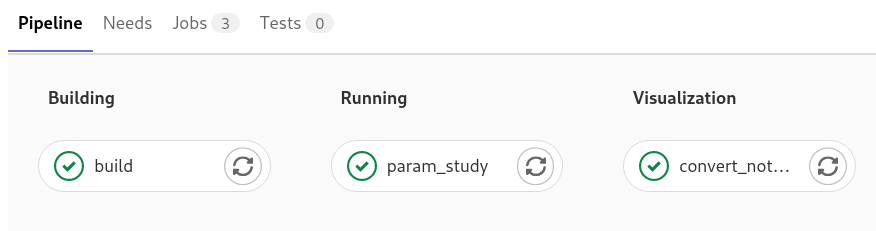
\includegraphics[width=0.6\textwidth]{figures/mwe-pipeline.png}

\end{frame}
